\documentclass[11pt]{report}
\usepackage{graphicx,multicol}
\usepackage[hidelinks]{hyperref}
%\usepackage[Glenn]{fncychap}  % Custom chapter style
\usepackage[english]{babel}
\usepackage{fancyhdr}
\pagestyle{fancy}
\usepackage{colortbl}
\usepackage[utf8]{inputenc}
\usepackage{amsmath}
\usepackage{geometry}
\usepackage{tikz}
\usepackage{setspace}
\usepackage{csquotes}
\setlength{\headheight}{13.6pt}

\usepackage{booktabs}
\usepackage{multicol}
\usepackage{float}
\usepackage{tocloft} 
\usepackage[backend=biber,style=apa]{biblatex}
\usepackage{booktabs} % For professional looking tables
\usepackage{tabularx} % For flexible column widths
\geometry{margin=1in}
\begin{document}


%
The maps in this section show the R-SQUARED between observed and modeled surface temperatures across the MENA region for the four seasons: JJA, DJF, MAM, and SON. R-SQUARED is a statistical measure that indicates how well the model explains the variability in observed data, with values closer to 1 signifying better performance. These maps provide valuable insights into the predictive skill of the climate models, highlighting their ability to capture seasonal temperature patterns.

\begin{figure}[H]
    \centering
    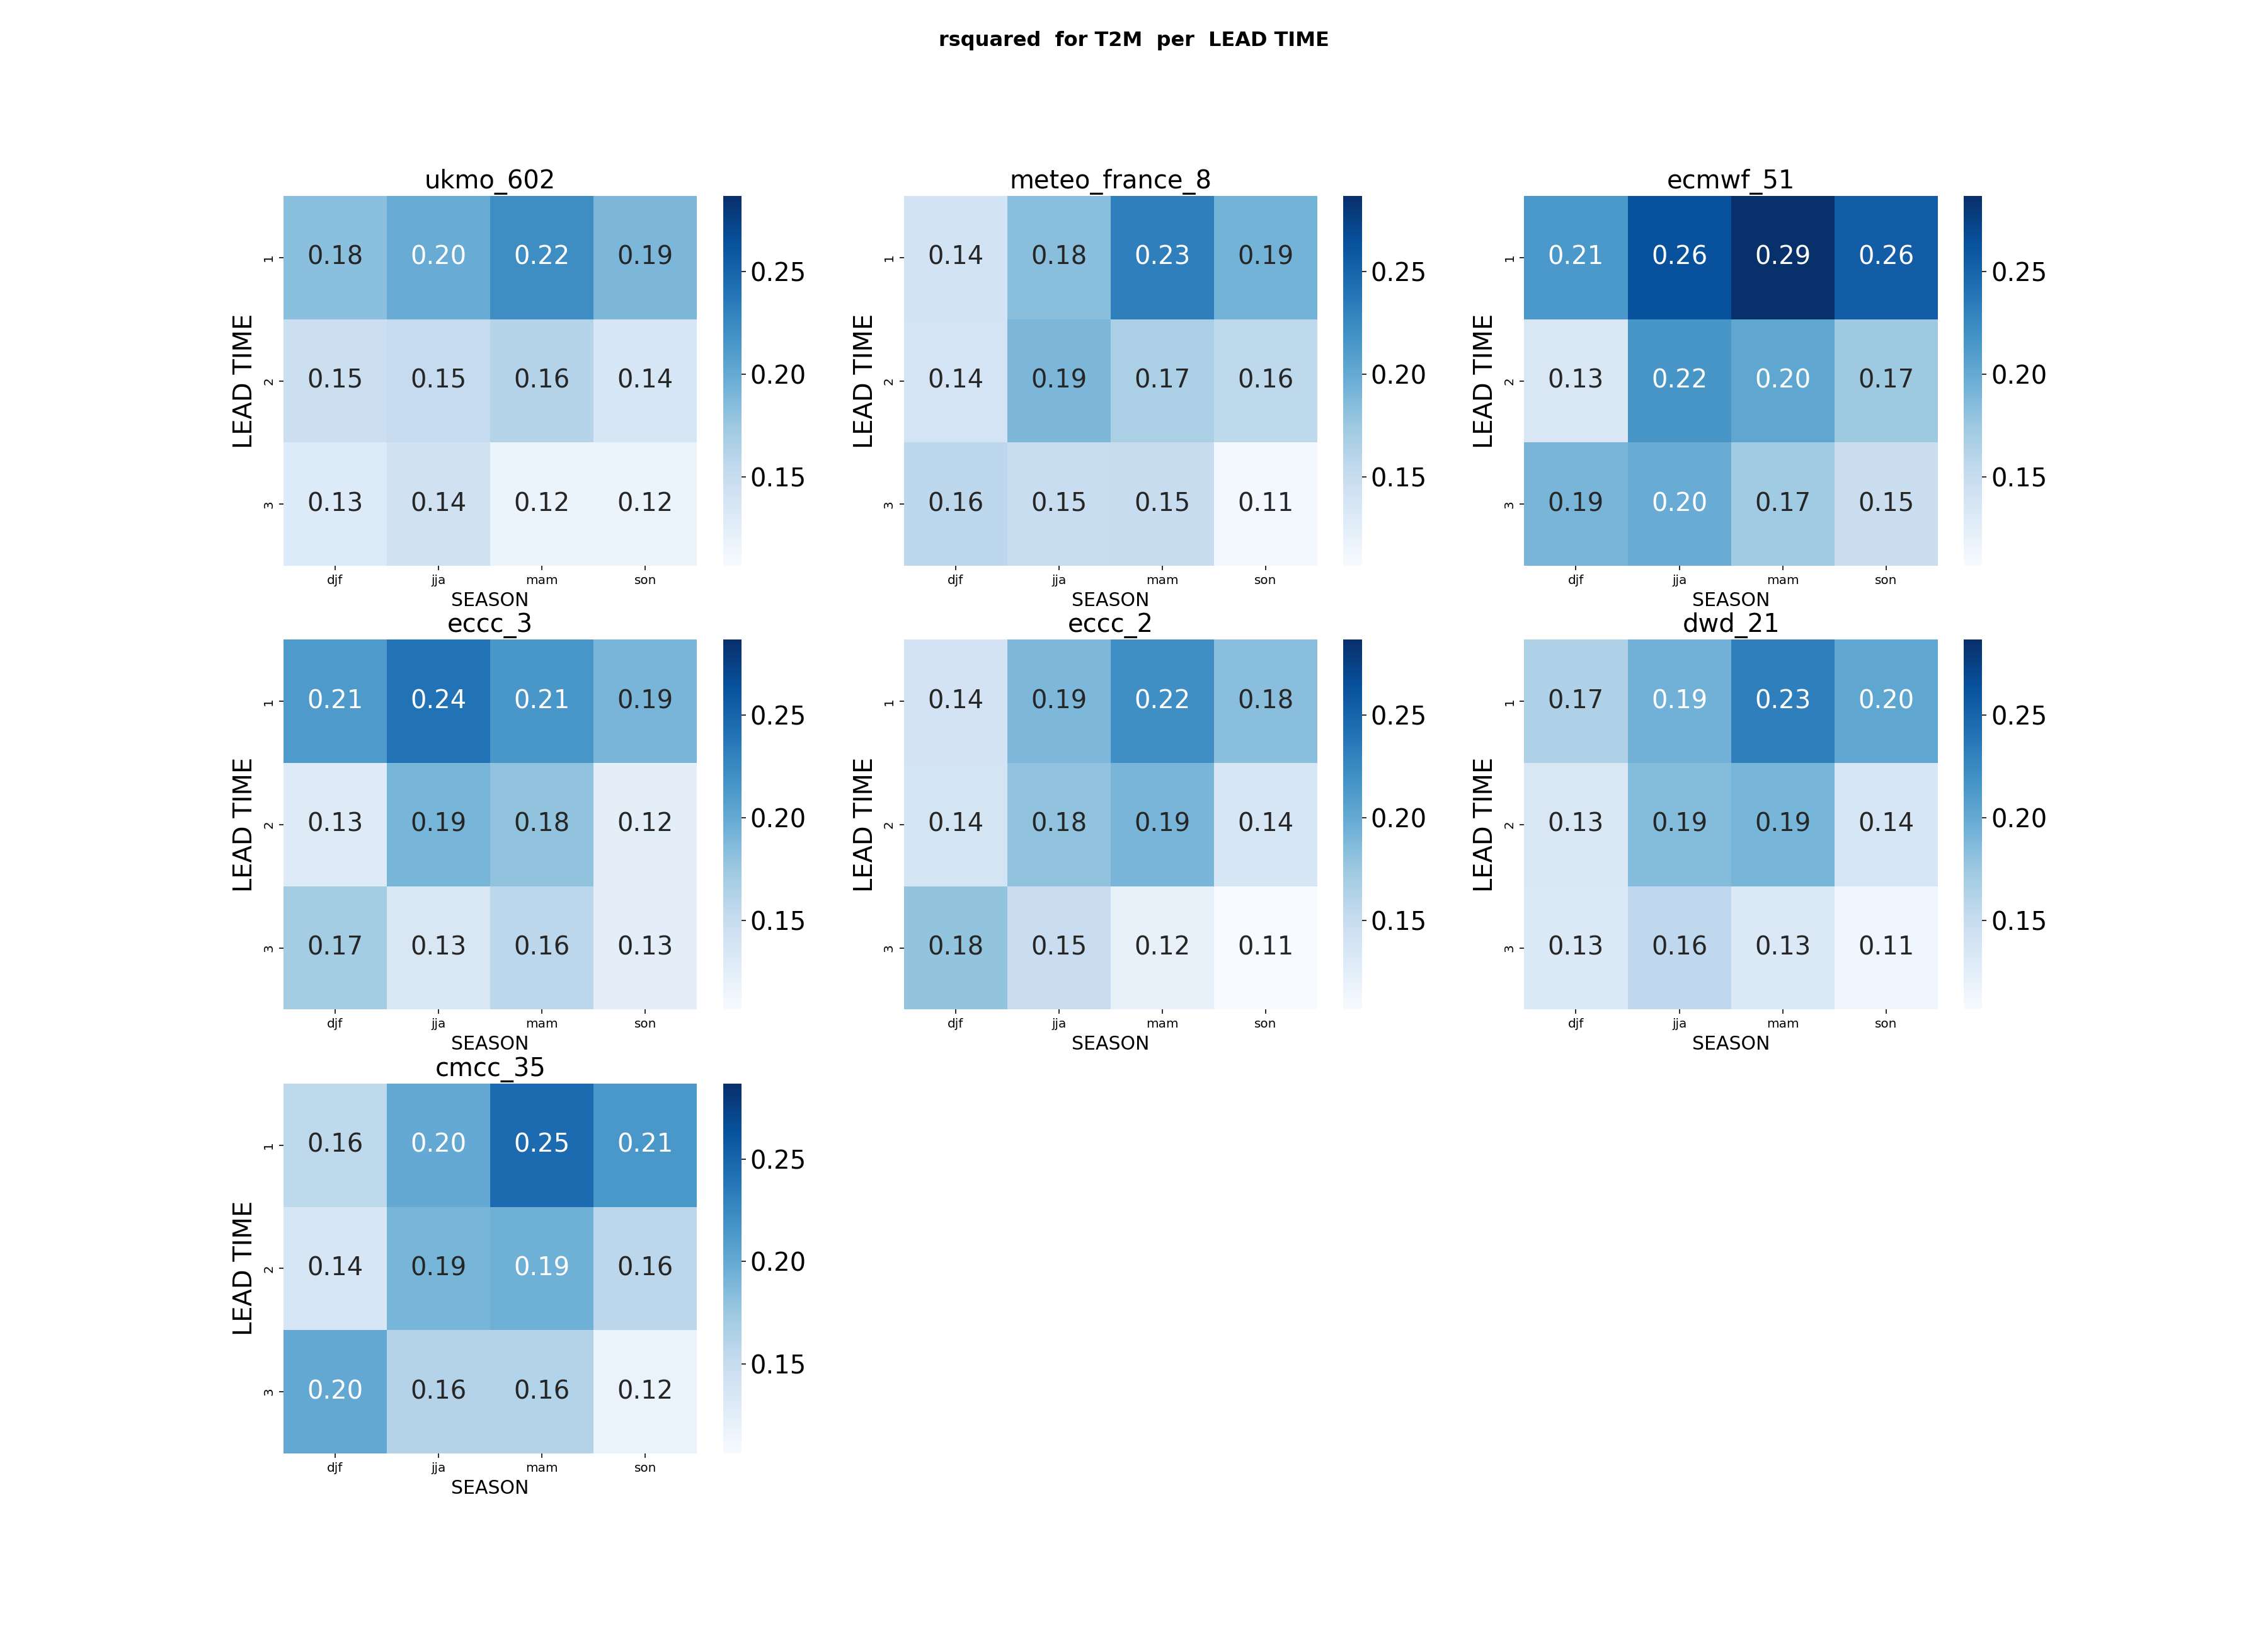
\includegraphics[scale=0.5]{plots/det/rsquared/rsquared_T2M.png}
    \caption{Temperature rsquared heatmaps for all the seasons}
\end{figure}

Based on this deterministic metric (R-SQUARED), the ECMWF model demonstrates superior performance for lead time 1 across all four seasons, particularly during MAM. In general, the portion of variance explained by the model decreases as the lead time increases. This indicates that while the model is highly effective at capturing seasonal variability of surface temperatures in the short term, its predictive skill diminishes over longer time horizons.
%
The strong performance during MAM highlights the ECMWF ability to capture the complexities of spring, a season marked by transitional weather patterns in the MENA region. The high R-SQUARED values during this period suggest that the model accurately reflects observed temperature variability by effectively simulating key drivers such as the gradual warming trend, atmospheric circulation changes, and the interaction between desert and coastal dynamics.
%
Such precision underscores the ECMWF model's reliability for short-term seasonal forecasting, particularly during periods of heightened climatic variability like MAM. However, the decreasing performance with increasing lead times suggests the need for careful interpretation of forecasts beyond lead time 1, as uncertainty increases with longer projections.
%
%\begin{figure}[H]
%    \centering
%    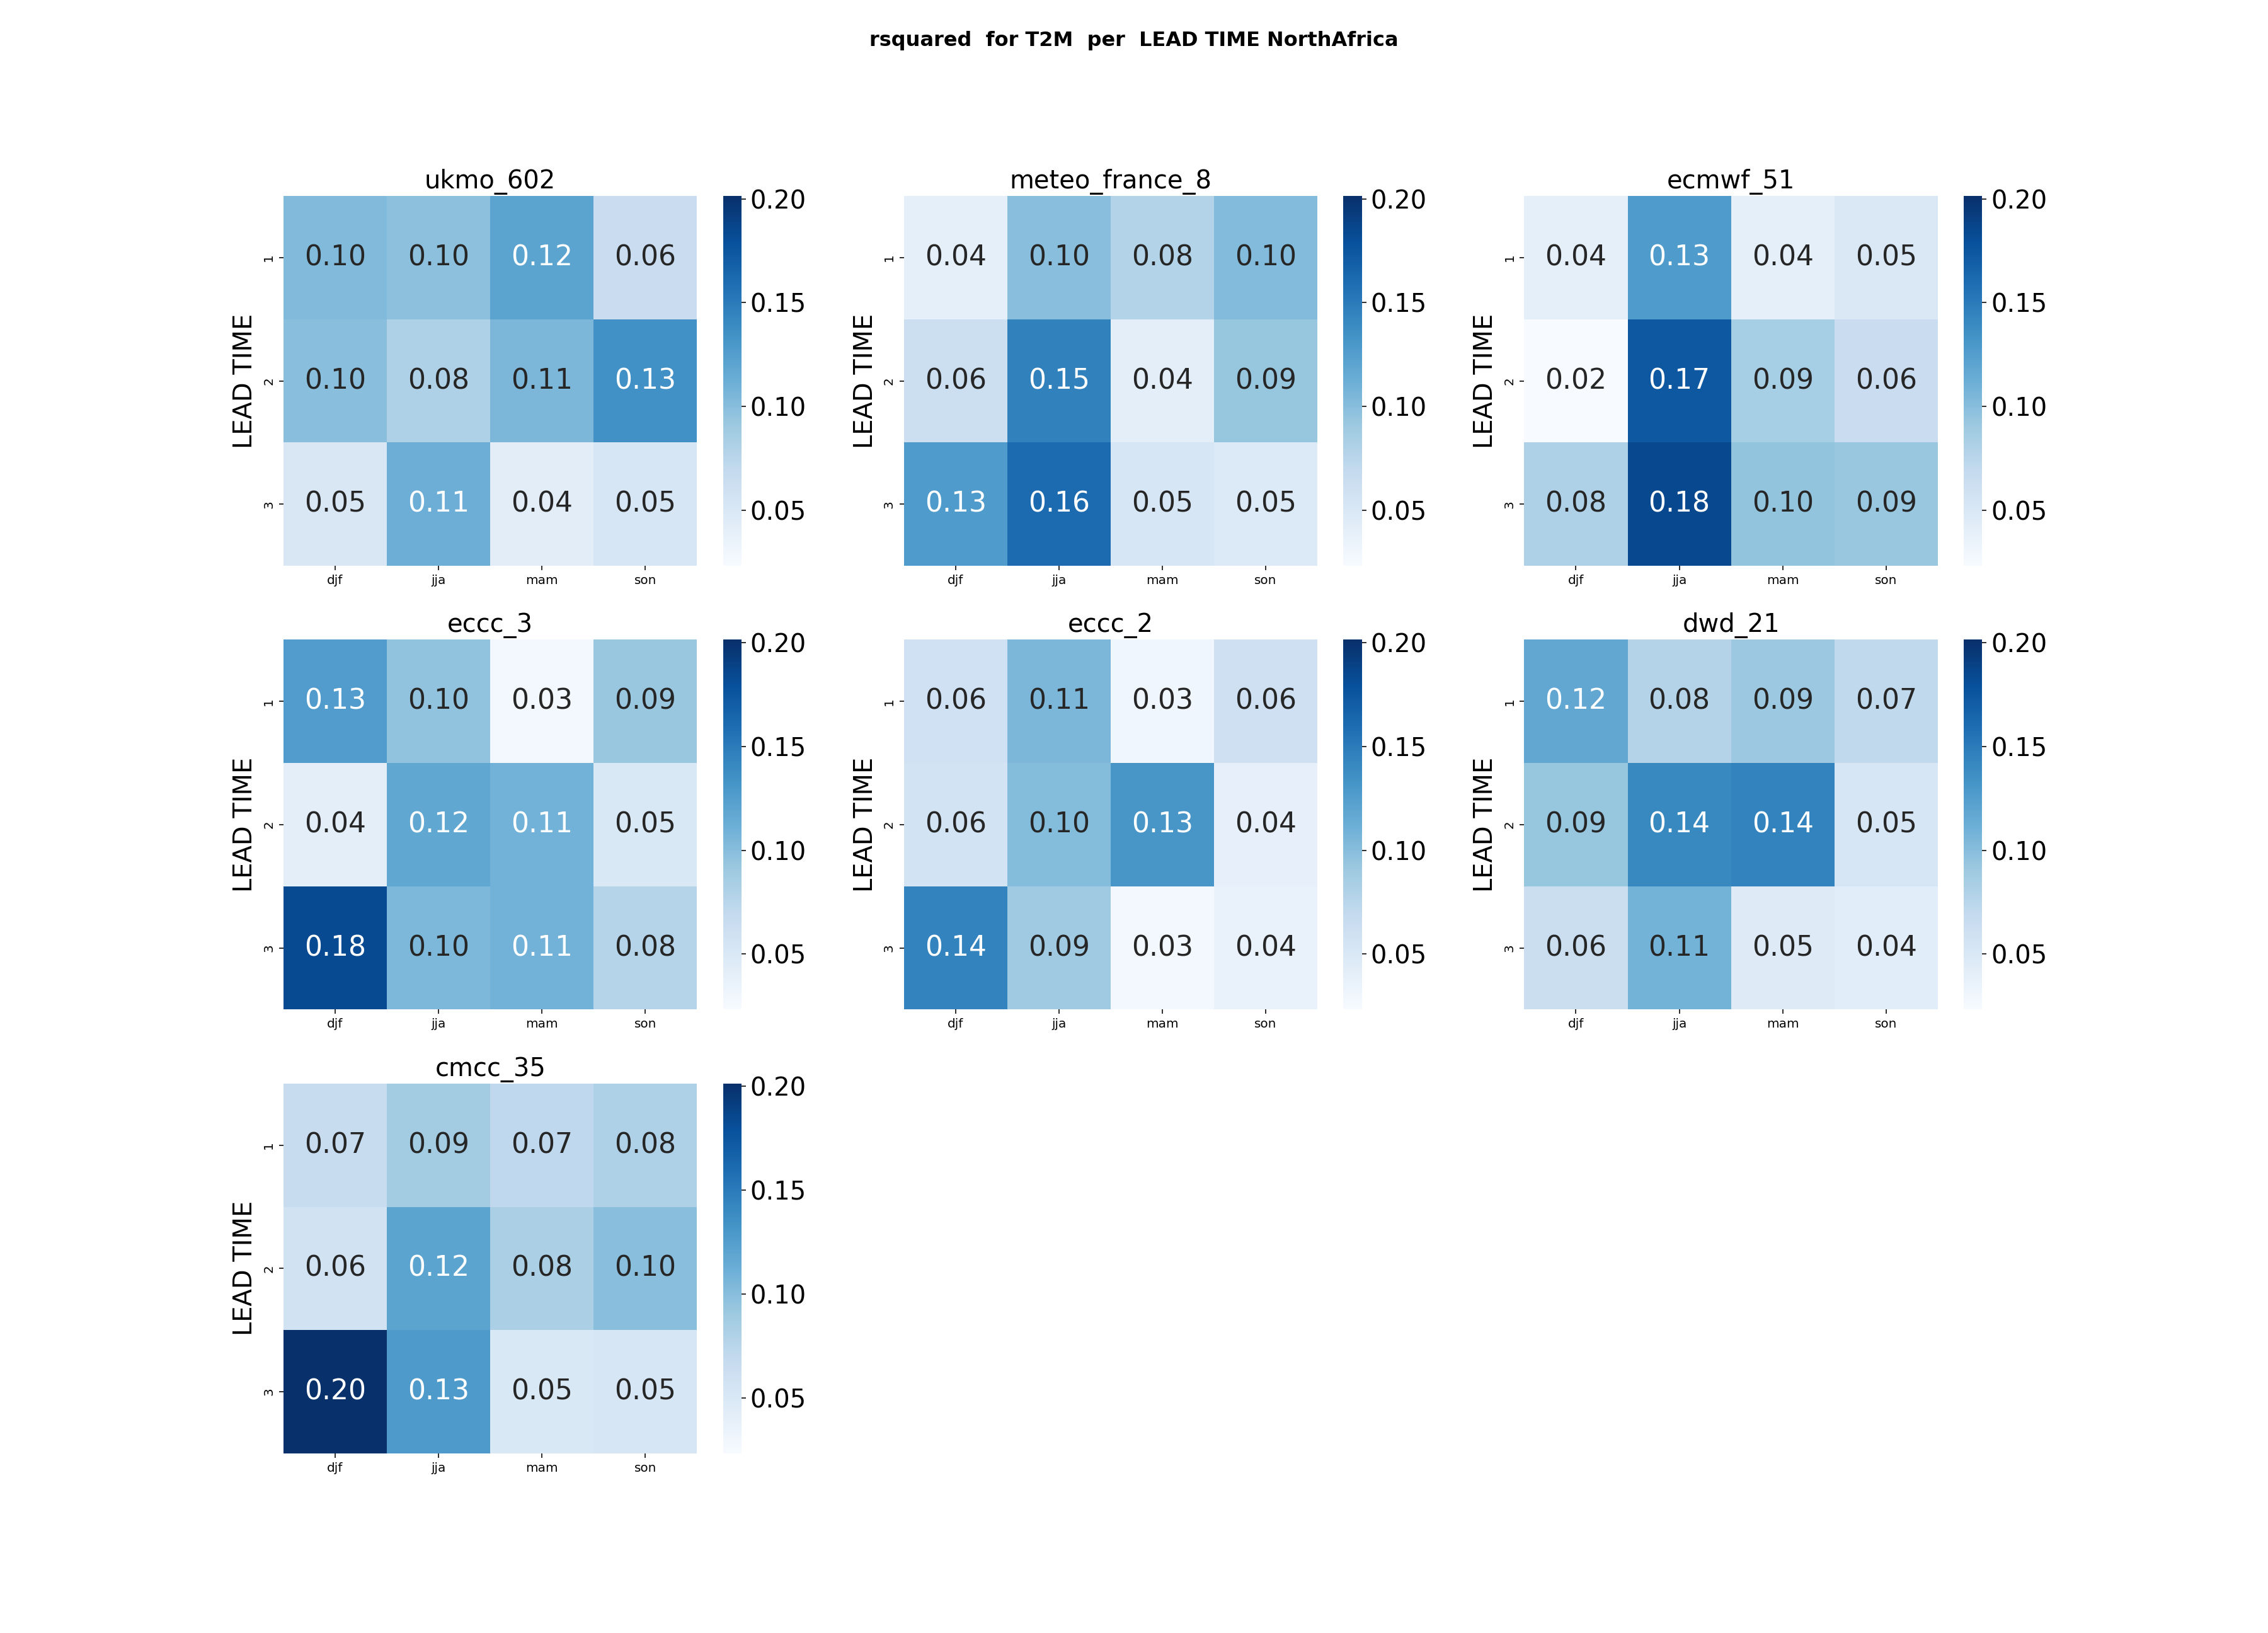
\includegraphics[scale=0.3]{plots/det/rsquared/rsquared_T2M_NorthAfrica.png}
%    \caption{2 meter temperature for North Africa}
%\end{figure}

\begin{figure}[H]
    \centering
    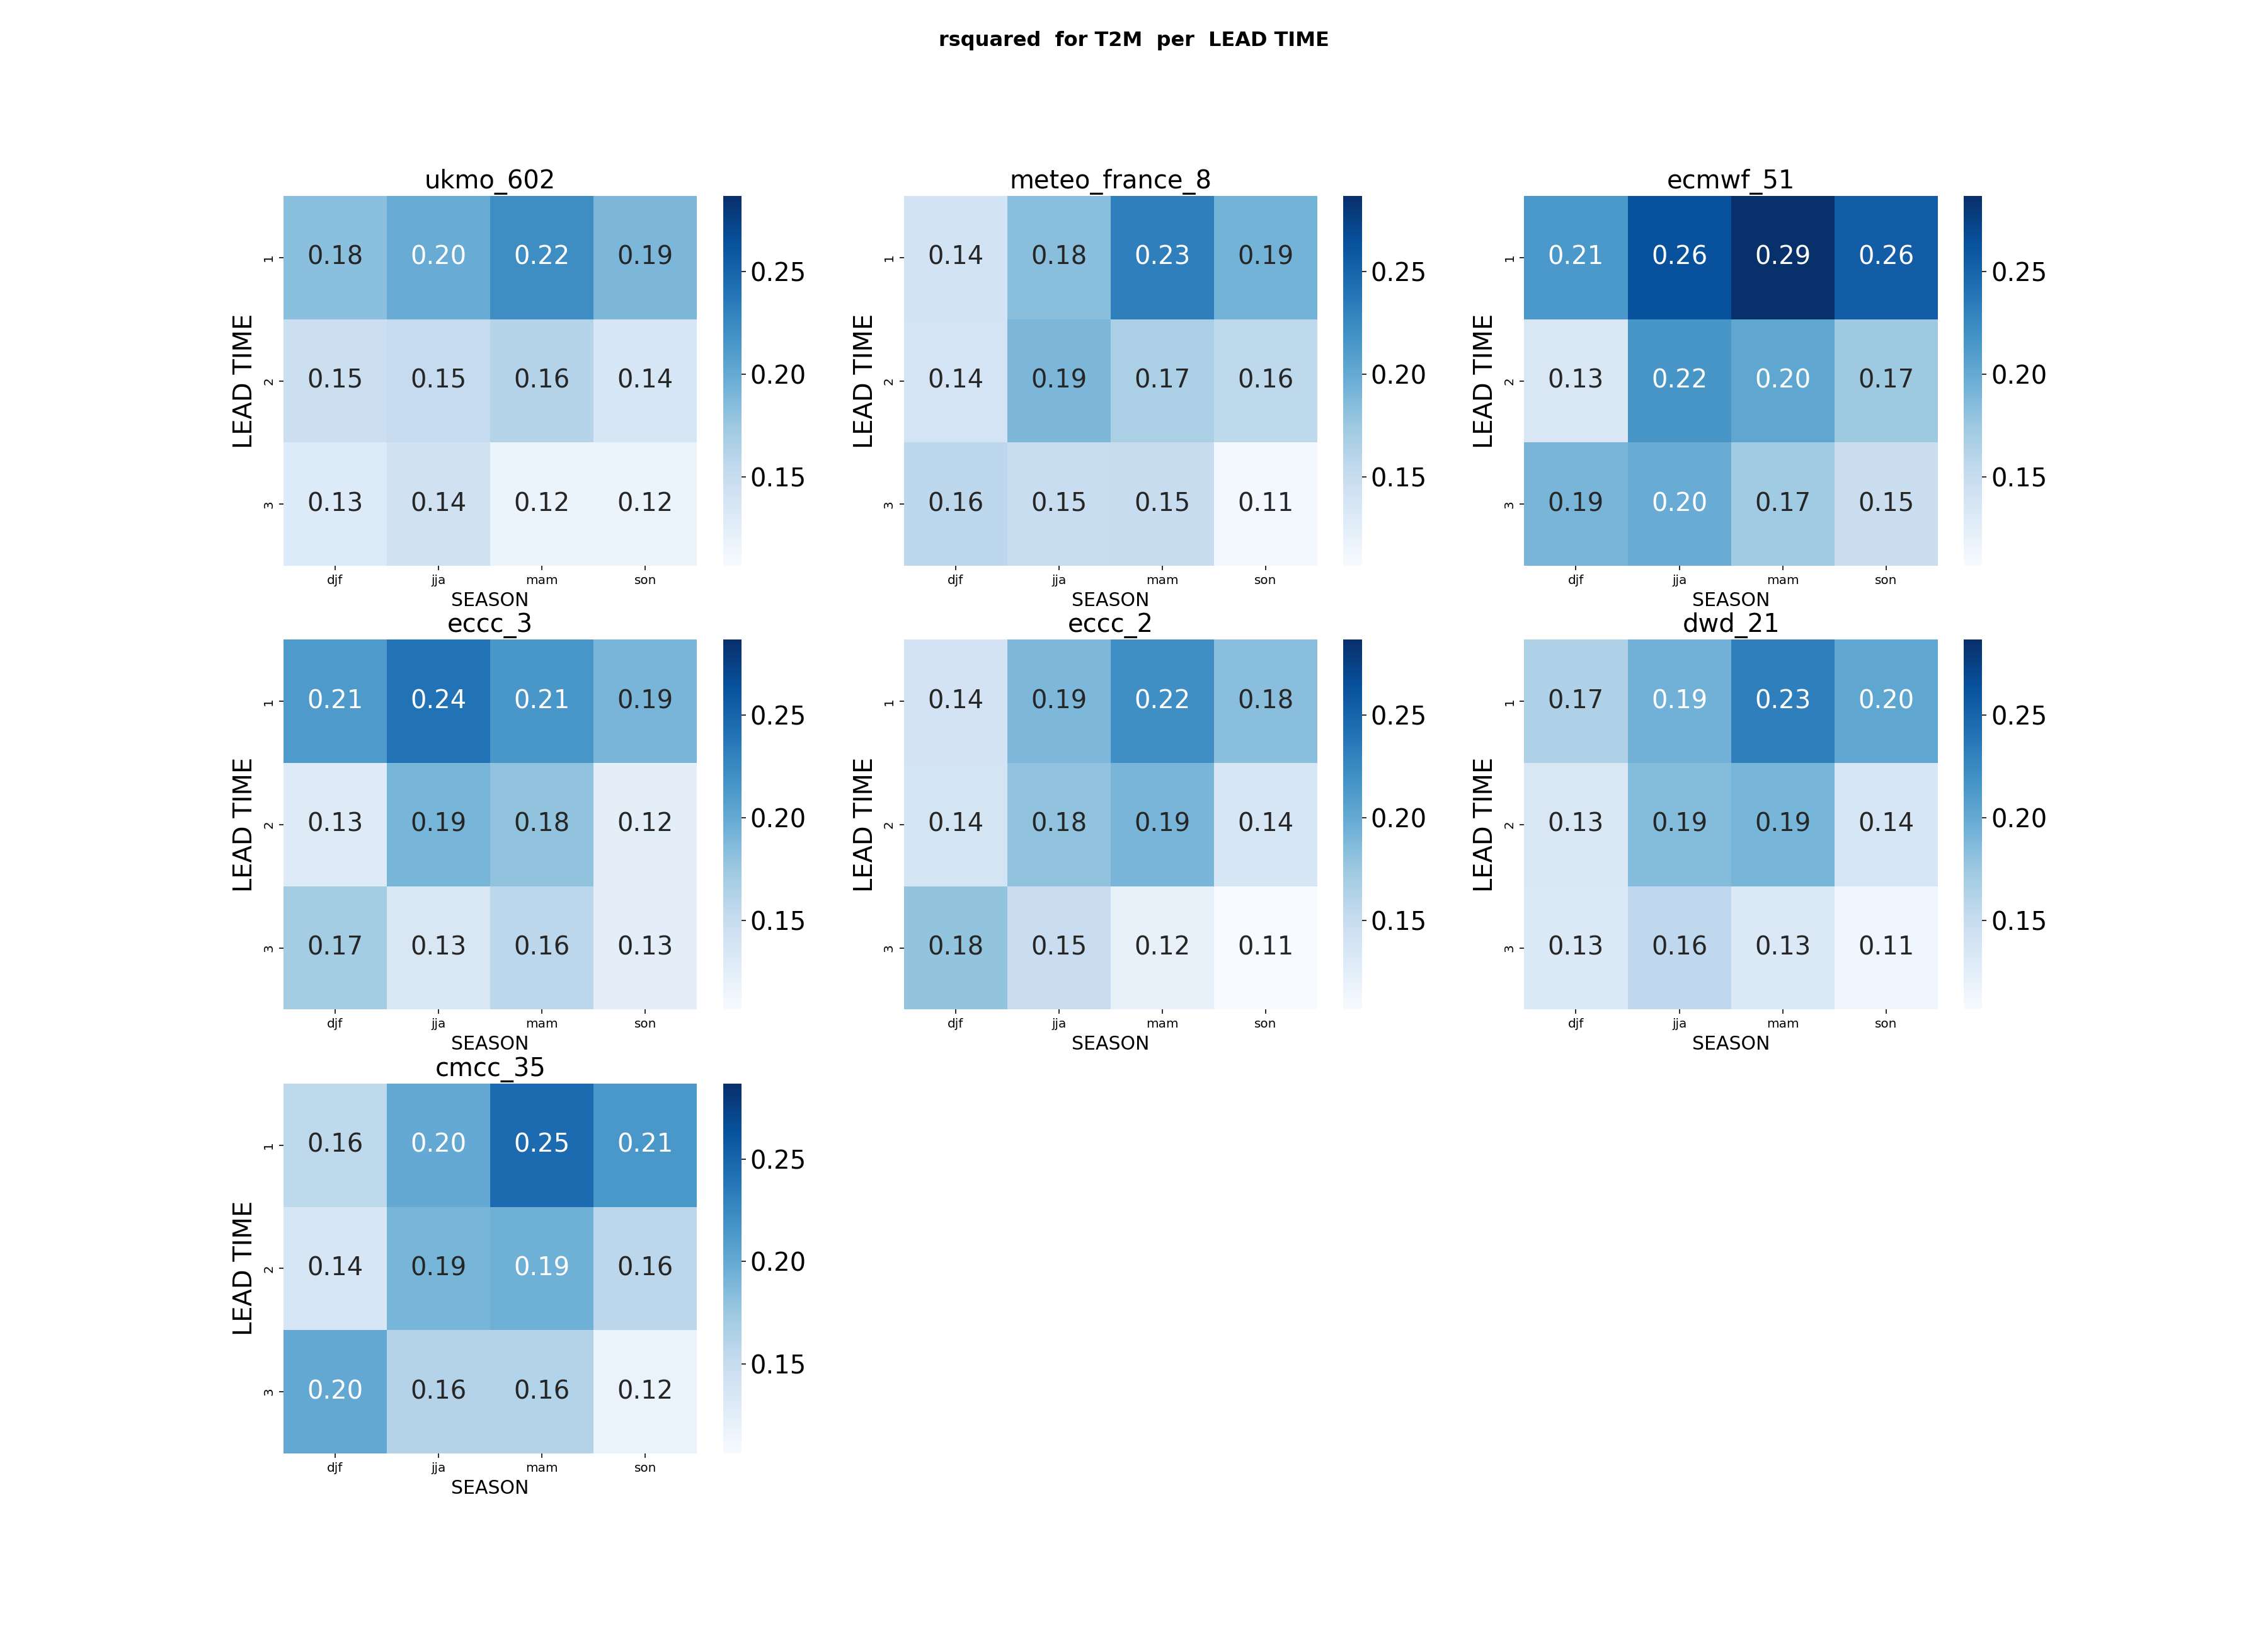
\includegraphics[scale=0.5]{plots/det/rsquared/rsquared_T2M.png}
    \caption{Temperature rsquared heatmaps for all the seasons NA}
\end{figure}

%A closer look at North Africa reveals that the ECMWF model performs best during JJA, with R-SQUARED values increasing as the lead time increases-contrary to the trend observed for the MENA region as a whole, where performance typically decreases with longer lead times. This suggests that the ECMWF model is particularly adept at capturing the persistent summer temperature patterns in North Africa, which may benefit from stronger model predictability over time due to the relatively stable atmospheric and climatic conditions during JJA.
%
%Similarly, Météo-France also shows good performance in North Africa, maintaining consistent R-SQUARED values across different lead times and seasons. This consistency highlights the model’s ability to handle the diverse climatic features of the region, such as the extreme temperatures influenced by the Sahara Desert and the moderating effects of the Mediterranean coastline.
%
%These findings emphasize the importance of regional analysis, as the performance of climate models can vary significantly within sub-regions of MENA. While ECMWF excels in predicting North Africa’s summer temperatures, the observed increase in R-SQUARED with lead time underscores the need to investigate the underlying factors driving this unusual trend, which contrasts with the broader MENA region's dynamics.
\end{document}